\textbf{Motivation.} In this section we describe the processes of Authentication and Authorization in the system.
It is worth to remember the meaning of Authentication and Authorization definitions.
Authentication -- is the process of ascertaining that somebody really is who they claim to be [\cite{burrows1989logic}].
Authorization refers to rules that determine who is allowed to do what [\cite{fagin1978authorization}].
For example, Adam may be authorized to create and delete databases, while Catherine is only authorized to read.
The two concepts are completely orthogonal and independent, but both are central to security design, and the
failure to get either one correct opens up the avenue to compromise.
In terms of web apps, very crudely speaking, authentication is when you check login credentials to see if you recognize
a user as logged in, and authorization is when you look up in your access control whether you allow the user to view,
edit, delete or create content.
Currently, there are two widely-known authentication methods, that are cookie authentication and JWT authentication.
We discuss JWTs straightforward.

\textbf{JWT Tokens.}
JSON Web Token (JWT) is an open standard [\cite{jones2015rfc}] that defines a compact and self-contained way for securely
transmitting information between parties as a JSON object [\cite{jones2015json}].
This information can be verified and trusted because it is digitally signed.
JWTs can be signed using a secret with the HMAC [\cite{wang2004hmac}] algorithm or a public/private key pair using
RSA [\cite{wiener1990cryptanalysis}] or ECDSA [\cite{johnson2001elliptic}].

Although JWTs can be encrypted to also provide secrecy between parties, we will focus on signed tokens.
Signed tokens can verify the integrity of the claims contained within it, while encrypted tokens hide those claims from
other parties.
When tokens are signed using public/private key pairs, the signature also certifies that only the party holding the
private key is the one that signed it.

When should you use JSON Web Tokens?

Here are some scenarios where JSON Web Tokens are useful:

\begin{itemize}
    \item \textbf{Authorization.} This is the most common scenario for using JWT. Once the user is logged in, each
    subsequent request will include the JWT, allowing the user to access routes, services, and resources that are permitted
    with that token.
    Single Sign On is a feature that widely uses JWT nowadays, because of its small overhead and its ability to be easily
    used across different domains.
    \item \textbf{Information Exchange.} JSON Web Tokens are a good way of securely transmitting information between
    parties.
    Because JWTs can be signed -- for example, using public/private key pairs -- you can be sure the senders are who they
    say they are.
    Additionally, as the signature is calculated using the header and the payload, you can also verify that the content
    hasn't been tampered with.
\end{itemize}

What is the JSON Web Token structure?
In its compact form, JSON Web Tokens consist of three parts separated by dots, which are Header, Payload, Signature.
Therefore, a JWT typically looks like
\begin{center}
    \begin{spverbatim}
        eyJhbGciOiJIUzI1NiIsInR5cCI6IkpXVCJ9.
        eyJzdWIiOiIxMjM0NTY3ODkwIiwibmFtZSI6I
        kpvaG4gRG9lIiwiaWF0IjoxNTE2MjM5MDIyfQ.
        SflKxwRJSMeKKF2QT4fwpMeJf36POk6yJV_adQ
        ssw5c
    \end{spverbatim}
\end{center}
Let's break down the different parts.
\begin{itemize}
    \item \textbf{Header.} Typically consists of two parts: the type of the token, which is JWT, and the signing algorithm
    being used, such as HMAC SHA256 or RSA\@.
    For example,

    \begin{spverbatim}
    {
        "alg": "HS256",
        "typ": "JWT"
    }
    \end{spverbatim}

    Then, this JSON is \href{https://en.wikipedia.org/wiki/Base64}{Base64Url} encoded to form the first part of the JWT\@.
    \item \textbf{Payload.} The second part of the token is the payload, which contains the claims.
    Claims are statements about an entity (typically, the user) and additional data.
    There are three types of claims: registered, public, and private claims.
    \begin{itemize}
        \item \textbf{Registered claims.} These are a set of predefined claims which are not mandatory but recommended,
        to provide a set of useful, interoperable claims.
        Some of them are: \textbf{iss} (issuer), \textbf{exp} (expiration time), \textbf{sub} (subject),
        \textbf{aud} (audience), and \href{https://tools.ietf.org/html/rfc7519#section-4.1}{others}.
        Notice that the claim names are only three characters long as JWT is meant to be compact.
        \item \textbf{Public claims.} These can be defined at will by those using JWTs. But to avoid collisions they
        should be defined in the \href{https://www.iana.org/assignments/jwt/jwt.xhtml}{IANA JSON Web Token Registry}
        or be defined as a URI that contains a collision resistant namespace.
        \item \textbf{Private claims.} These are the custom claims created to share information between parties that
        agree on using them and are neither registered or public claims.
    \end{itemize}
    An example payload could be:

    \begin{spverbatim}
    {
        "sub": "1234567890",
        "name": "John Doe",
        "admin": true
    }
    \end{spverbatim}

    The payload is then Base64Url encoded to form the second part of the JSON Web Token.
    Do note that for signed tokens this information, though protected against tampering, is readable by anyone.
    Do not put secret information in the payload or header elements of a JWT unless it is encrypted.
    \item \textbf{Signature.} To create the signature part you have to take the encoded header, the encoded payload, a secret,
    the algorithm specified in the header, and sign that.
    For example if you want to use the HMAC SHA256 algorithm, the signature will be created in the following way:

    \begin{spverbatim}
        HMACSHA256(
        base64UrlEncode(header) + "." +
        base64UrlEncode(payload),
        secret)
    \end{spverbatim}

    The signature is used to verify the message wasn't changed along the way, and, in the case of tokens signed
    with a private key, it can also verify that the sender of the JWT is who it says it is.
    \item \textbf{Putting all together.} The output is three Base64-URL strings separated by dots that can be easily
    passed in HTML and HTTP environments, while being more compact when compared to XML-based standards such as SAML\@.
    The following shows a JWT that has the previous header and payload encoded, and it is signed with a secret.

    \begin{spverbatim}
        eyJhbGciOiJIUzI1NiIsInR5cCI6IkpXVCJ9.
        eyJqdGkiOiJmZDNjNjdjNS1jNmZmLTRhNWQtY
        TE2Ni05OGVjZTFiNzc1MmIiLCJyb2xlIjoiVX
        NlciIsIm5iZiI6MTYzMTU1MjQ5NiwiZXhwIjo
        xNjMxNTUyNzk2LCJpYXQiOjE2MzE1NTI0OTYs
        ImlzcyI6Imh0dHBzOi8vbWFuZ28tbWVzc2VuZ
        2VyLWFwcC5oZXJva3VhcHAuY29tIiwiYXVkIj
        oiaHR0cHM6Ly9tYW5nby1tZXNzZW5nZXItYXB
        wLmhlcm9rdWFwcC5jb20vYXBpIn0.
        locHt8ow1lFnGGZ_aFFvXI09dD4y1r594XQF2
        -6YxCw
    \end{spverbatim}

\end{itemize}

As to the projects concerns, we should handle multiple client applications, e.g desktop,
web, mobile etc.
Therefore, HTTP cookie authorization doesn't fit our requirements, however the JWT one surely passes.

\textbf{JWT Authorization.} In authentication, when the user successfully logs in using their credentials, a JSON Web Token will be returned.
Since tokens are credentials, great care must be taken to prevent security issues.
In general, you should not keep tokens longer than required.
You also should not store sensitive session data in browser storage due to lack of security.
Whenever the user wants to access a protected route or resource, the user agent should send the JWT,
typically in the Authorization header using the Bearer schema.
The content of the header should look like the following:
\begin{spverbatim}

    Authorization: Bearer <token>

\end{spverbatim}
This can be, in certain cases, a stateless authorization mechanism.
The server's protected routes will check for a valid JWT in the Authorization header, and if it's present,
the user will be allowed to access protected resources.
If the JWT contains the necessary data, the need to query the database for certain operations may be reduced,
though this may not always be the case.
If the token is sent in the Authorization header, Cross-Origin Resource Sharing (CORS) won't be an issue
as it doesn't use cookies.
Generally, the workflow is as follows
% old
\begin{enumerate}
    \item User provides credentials in order to authenticate to the system.
    \item Server verifies user's authentication, fetches the login and password in database.
    \item If authentication is successful, server creates session then writes this session to the database,
    see table session in [REFERENCE\_DATABASE\_SCHEMA].
    \item Server generates a pair of access token (JWT) and refresh token (GUID).
    \item Server sends to client access token and refresh token.
    \item Client saves the pair of access and refresh tokens.
    \item User requests resource using received token passed to the request header.
    \item The server check user's claims and proceeds or declines request.
\end{enumerate}

The eighth point is the authorization.
As a result, token stored on the client and used when it is necessary to authorize the requests.
When a hacker tries to replace the data in the header or payload the token will become invalid,
therefore the signature will not match the original values.
So, the hacker hasn't any possibility to generate a new signature since that encryption secret key stored on the server.
Access token (JWT) is used for request authorization and for storing the additional information about user like identifier,
display name and others.
Refresh Token (GUID) issued by server based on successful authentication results and used for get new access/refresh
token pair.
Also, it is worth to add a few basic rules about JWT secure usage [\cite{RDegges}]
\begin{itemize}
    \item JWT should have a short lifetime, since it cannot be revoked.
    \item JWT should be used in a single time, e.g JWT per request.
\end{itemize}
Therefore, we consider access token's lifetime to be 5 minutes and refresh token's 7 days.

For each request client preliminarily checks access token's lifetime.
If access token it expired, client sends request for updating a pair of access/refresh tokens.
For more confidence, we can update tokens a few seconds earlier.
That is, the case when the API receives an expired access token is practically excluded.
However, we are able to consider the case of interception of the request on 401 http response code,
that is unauthorized.
The following diagram demonstrates the process of requesting the resource

\begin{figure}[H]
    \centering
    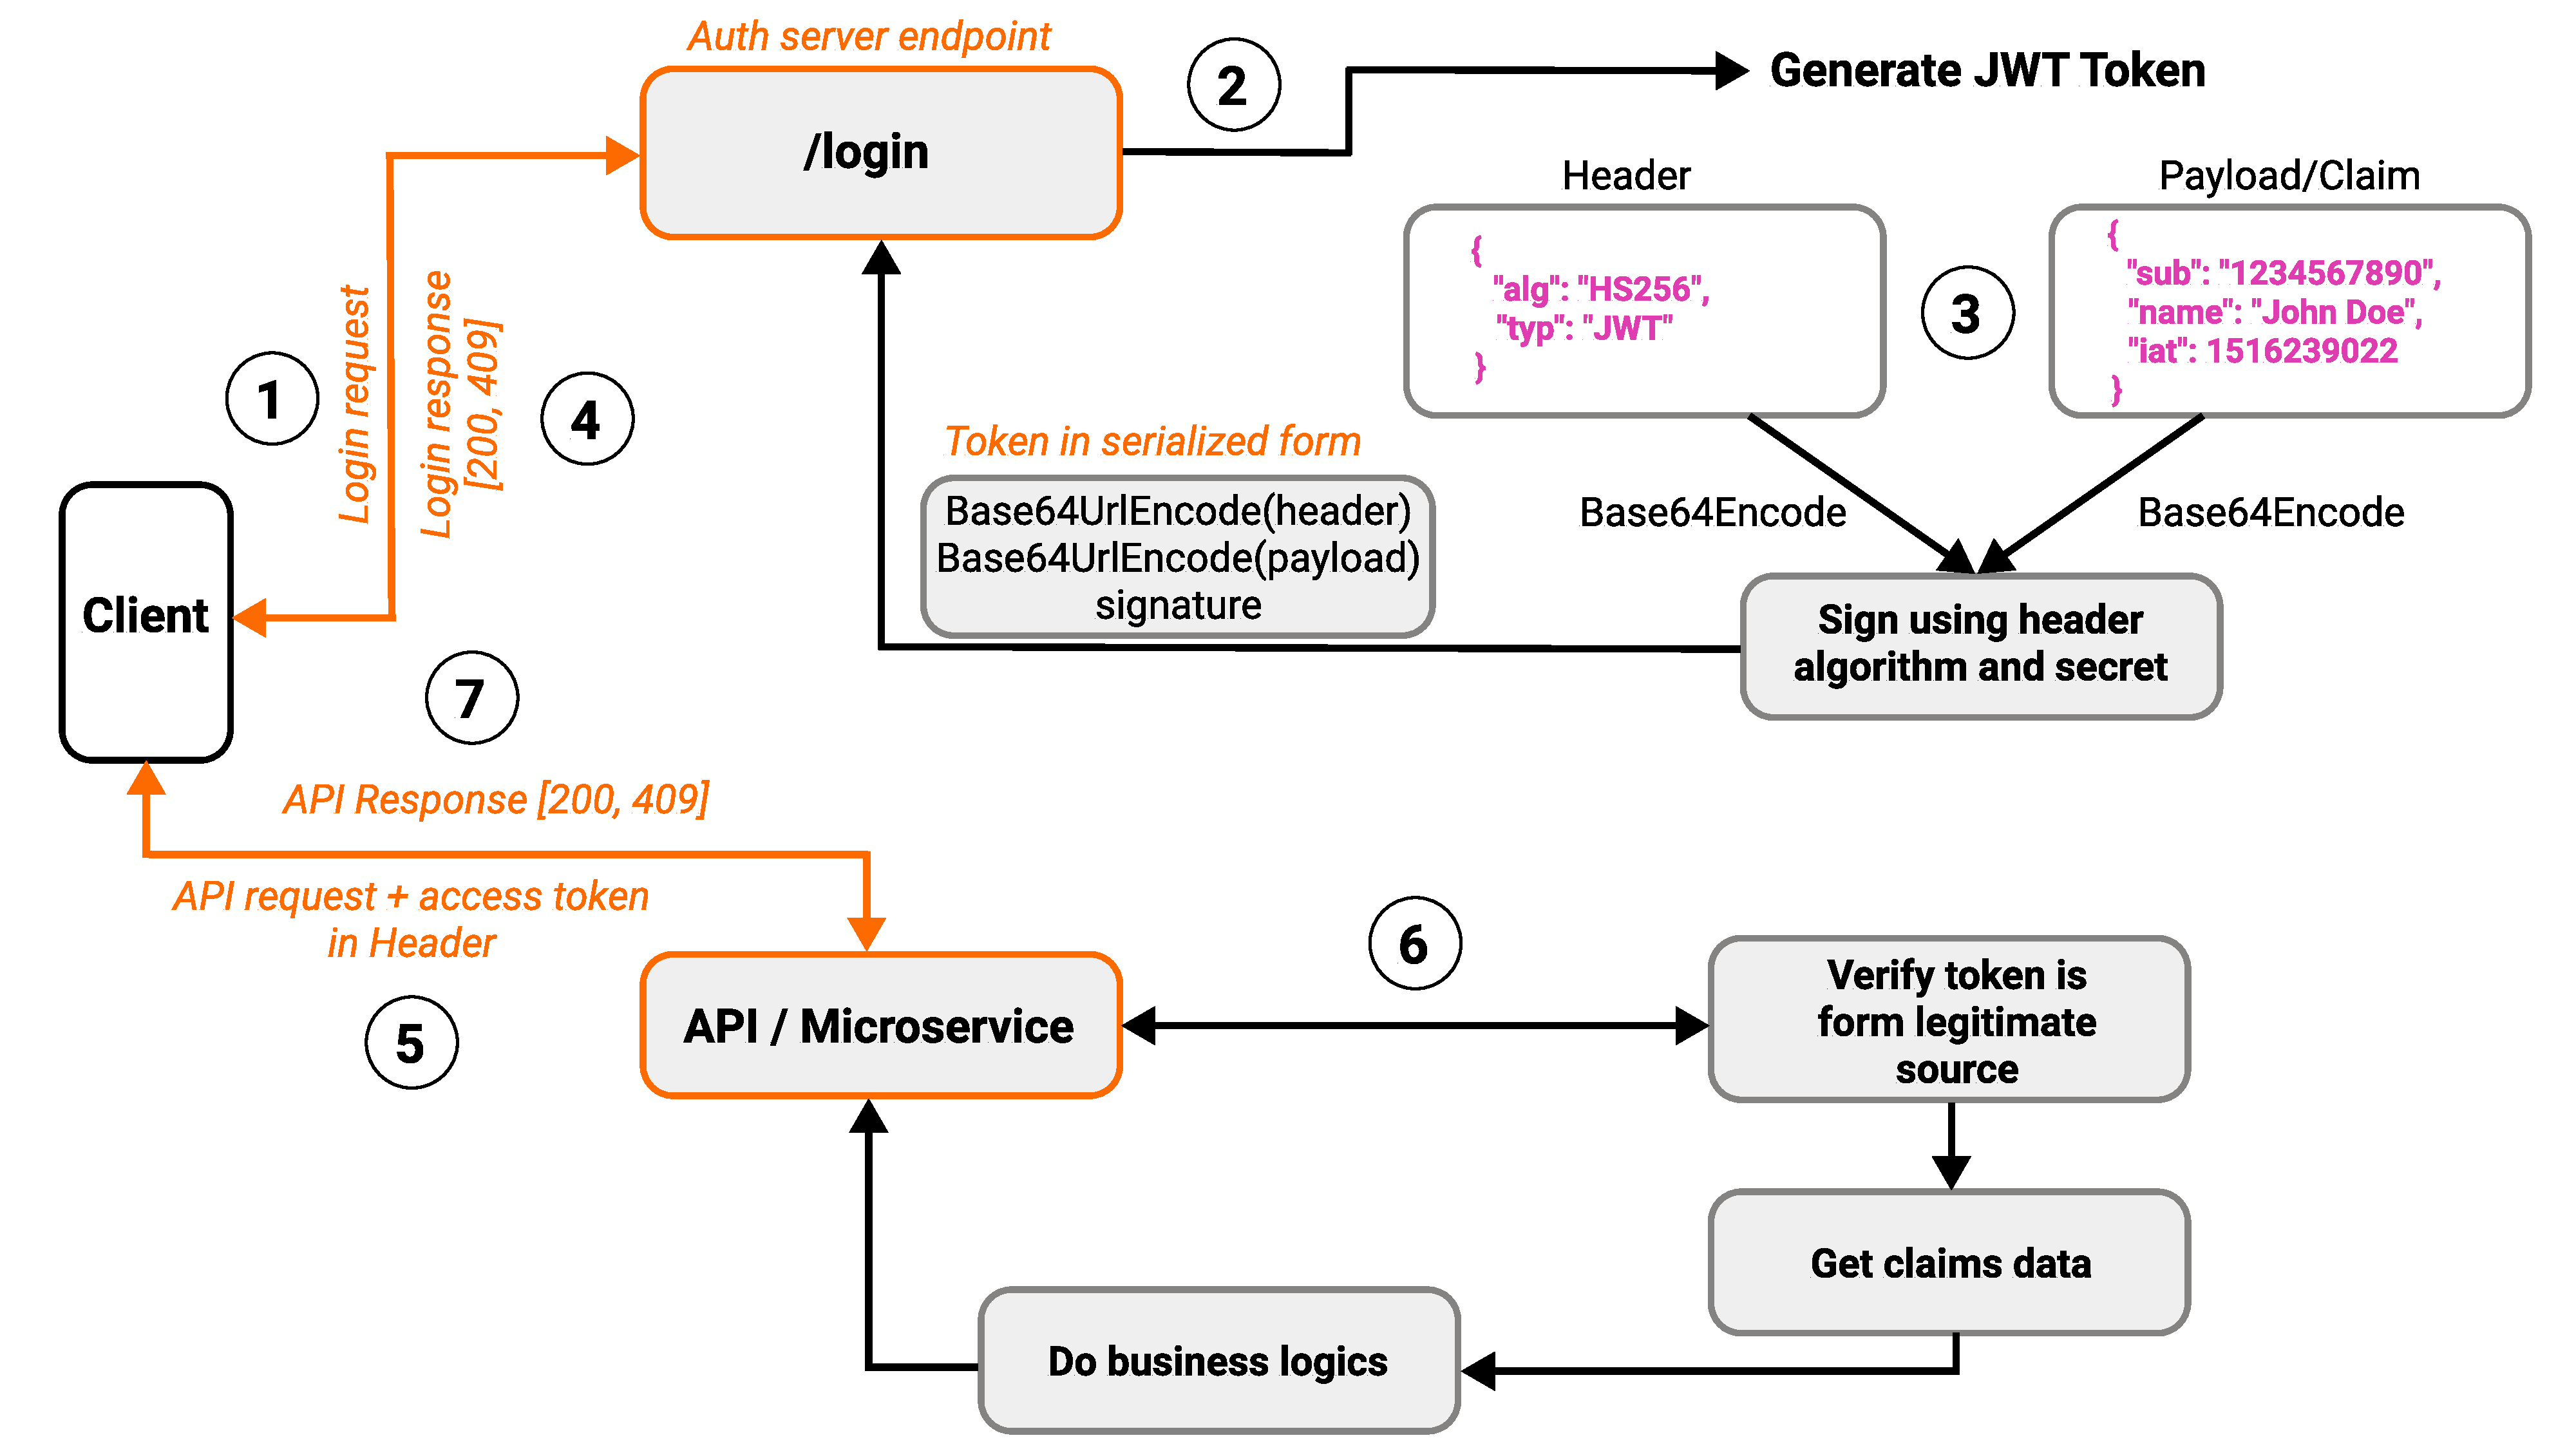
\includegraphics[width=1\textwidth]{Pictures/jwt_auth_scheme.pdf}
    \caption{JWT Authentication concept diagram.}\label{fig:figure3}
\end{figure}

By steps, the process is
\begin{itemize}
    \item \textbf{Step 1.} \textbf{Client} application sends \textbf{POST} authentication request to
    the \textbf{Auth server endpoint} provided user credentials in request body.
    \item \textbf{Step 2.} \textbf{Auth server endpoint} responses to the \textbf{Client} with the following HTTP response codes:
    \begin{itemize}
        \item \textbf{409Conflict}: Invalid credentials.
        \item \textbf{200Success}: Returns a pair of access and refresh tokens.
        \begin{itemize}
            \item \textbf{Step 3.} Server generates a pair of access and refresh tokens
            \begin{itemize}
                \item API fetches user data and claims.
                \item Server creates new session instance in database.
                \item Access token's \textbf{Header} Base64 encoded.
                \item Access token's \textbf{Payload} with user claims is Base64 encoded.
                \item Access token's \textbf{Signature} is generated using encoded token's Header and Payload signed by means of the
                algorithm (HMACSHA256) from the header and secret:
                \begin{spverbatim}
                    Signature = HMACSHA256(
                    base64UrlEncode(header) + "." +
                    base64UrlEncode(payload),
                    secret)
                \end{spverbatim}
            \end{itemize}
        \end{itemize}
    \end{itemize}
    \item \textbf{Step 4.} Access token in serialized form and refresh token (GUID) returned in response with
    HTTP \textbf{200Success} code to the \textbf{Client}.
    \item \textbf{Step 5.} \textbf{Client} queries the \textbf{API / Microservice} providing access token as
    \textbf{Bearer} in request header.
    \item \textbf{Step 6.} \textbf{API / Microservice} validates the token claims in order to authorize user
    \begin{itemize}
        \item If authorized: \textbf{API / Microservice} does business logics and returns response \textbf{(Step 7)}.
        \item Otherwise: returns \textbf{401Unauthorized} response code.
    \end{itemize}
    \item \textbf{Step 7.} \textbf{API / Microservice} returns response \textbf{200Success} or \textbf{409Conflict}
    to the client according to backend business logic.
\end{itemize}